% !TeX root = ../DistributedConsensus.tex
% !TeX spellcheck = en_GB
\chapter{Reducing Histories to Orders of Execution}
\label{chap:order-of-execution}
\section{Order of Execution}
	When a combined history has been produced, it represents every action that has occurred on all the events of the workflow. 
	Recall that the goal is to provide an order of execution and excess information in the history therefore needs to be removed in a way that still provides the same amount of information about the order of executions. By reducing the history to an order of execution a minimal equivalent graph is then achieved.\todo{maybe it is not equivalent since collapse actually removes info}
	
	\subsection{Collapsing}
	In definition \todo[inline]{lav label til definitions} we saw that an execution was defined to be all the action between an \texttt{execution start} and \texttt{execution finish} actions. Furthermore even though the receiver saves incoming actions, these actions are still initiated by the performer, and these actions can therefore be seen as being parts of the performers execution. 
	
	\newpar Due to the property of an execution stated in \todo[inline]{label math} which states that some actions might be concurrent with other actions even though it is possible to establish a happens before with some of the actions. Therefore we need to make an assumption which states that everything in an execution happens at the same time and therefore any happens before relations  any action has with any actions outside of the execution is now present on all the events in the execution. When this is the case, every action inside the execution are equal in terms of happens before relations and therefore we can \textit{collapse} the execution into one single action.
	
	The assumption that every action of an execution are concurrent and have the same happens before relation as any other action, holds true when it is taken into consideration that the events execute serially equivalent, meaning that an incoming action must happen after and before any actions from other executions. 
		
%	\newpar It is necessary to determine what should represent the time of an execution. Possible candidates would be \texttt{ExecuteFinish} and \texttt{ExecuteStart}. Using \texttt{ExecuteFinish}, it is difficult to tell which execution happened before the other, due to the fact that actions that are part of an execution happen before the \texttt{ExecuteFinish} action. 
%	The same applies for the \texttt{ExecuteStart} action, where actions that are part of an execution can happen after the execution.
	
	\newpar It then is necessary to research a way to \textit{collapse} an execution in order to overcome these problems. \textit{Collapsing} constitutes looking at all actions between an \texttt{ExecuteStart} action and an \texttt{ExecuteFinish} action of an event and connecting these events into a single entity, representing an entire execution. 
	
	Actions between start and finish might contain relations to other actions located in the local histories of other events. Since a given event is only affected by the effects of other events executing, it is safe to collapse the incoming actions from executing events into execution of the executing event. Since an action is always caused by the execution of \textit{some} event, the collapsed execution has the property that no action can happened outside any collapsed execution.
	
	An example of this separation of executions can be found in \autoref{fig:orderofexecution:collapsing}.
	
	\begin{figure}[H]
		\centering
		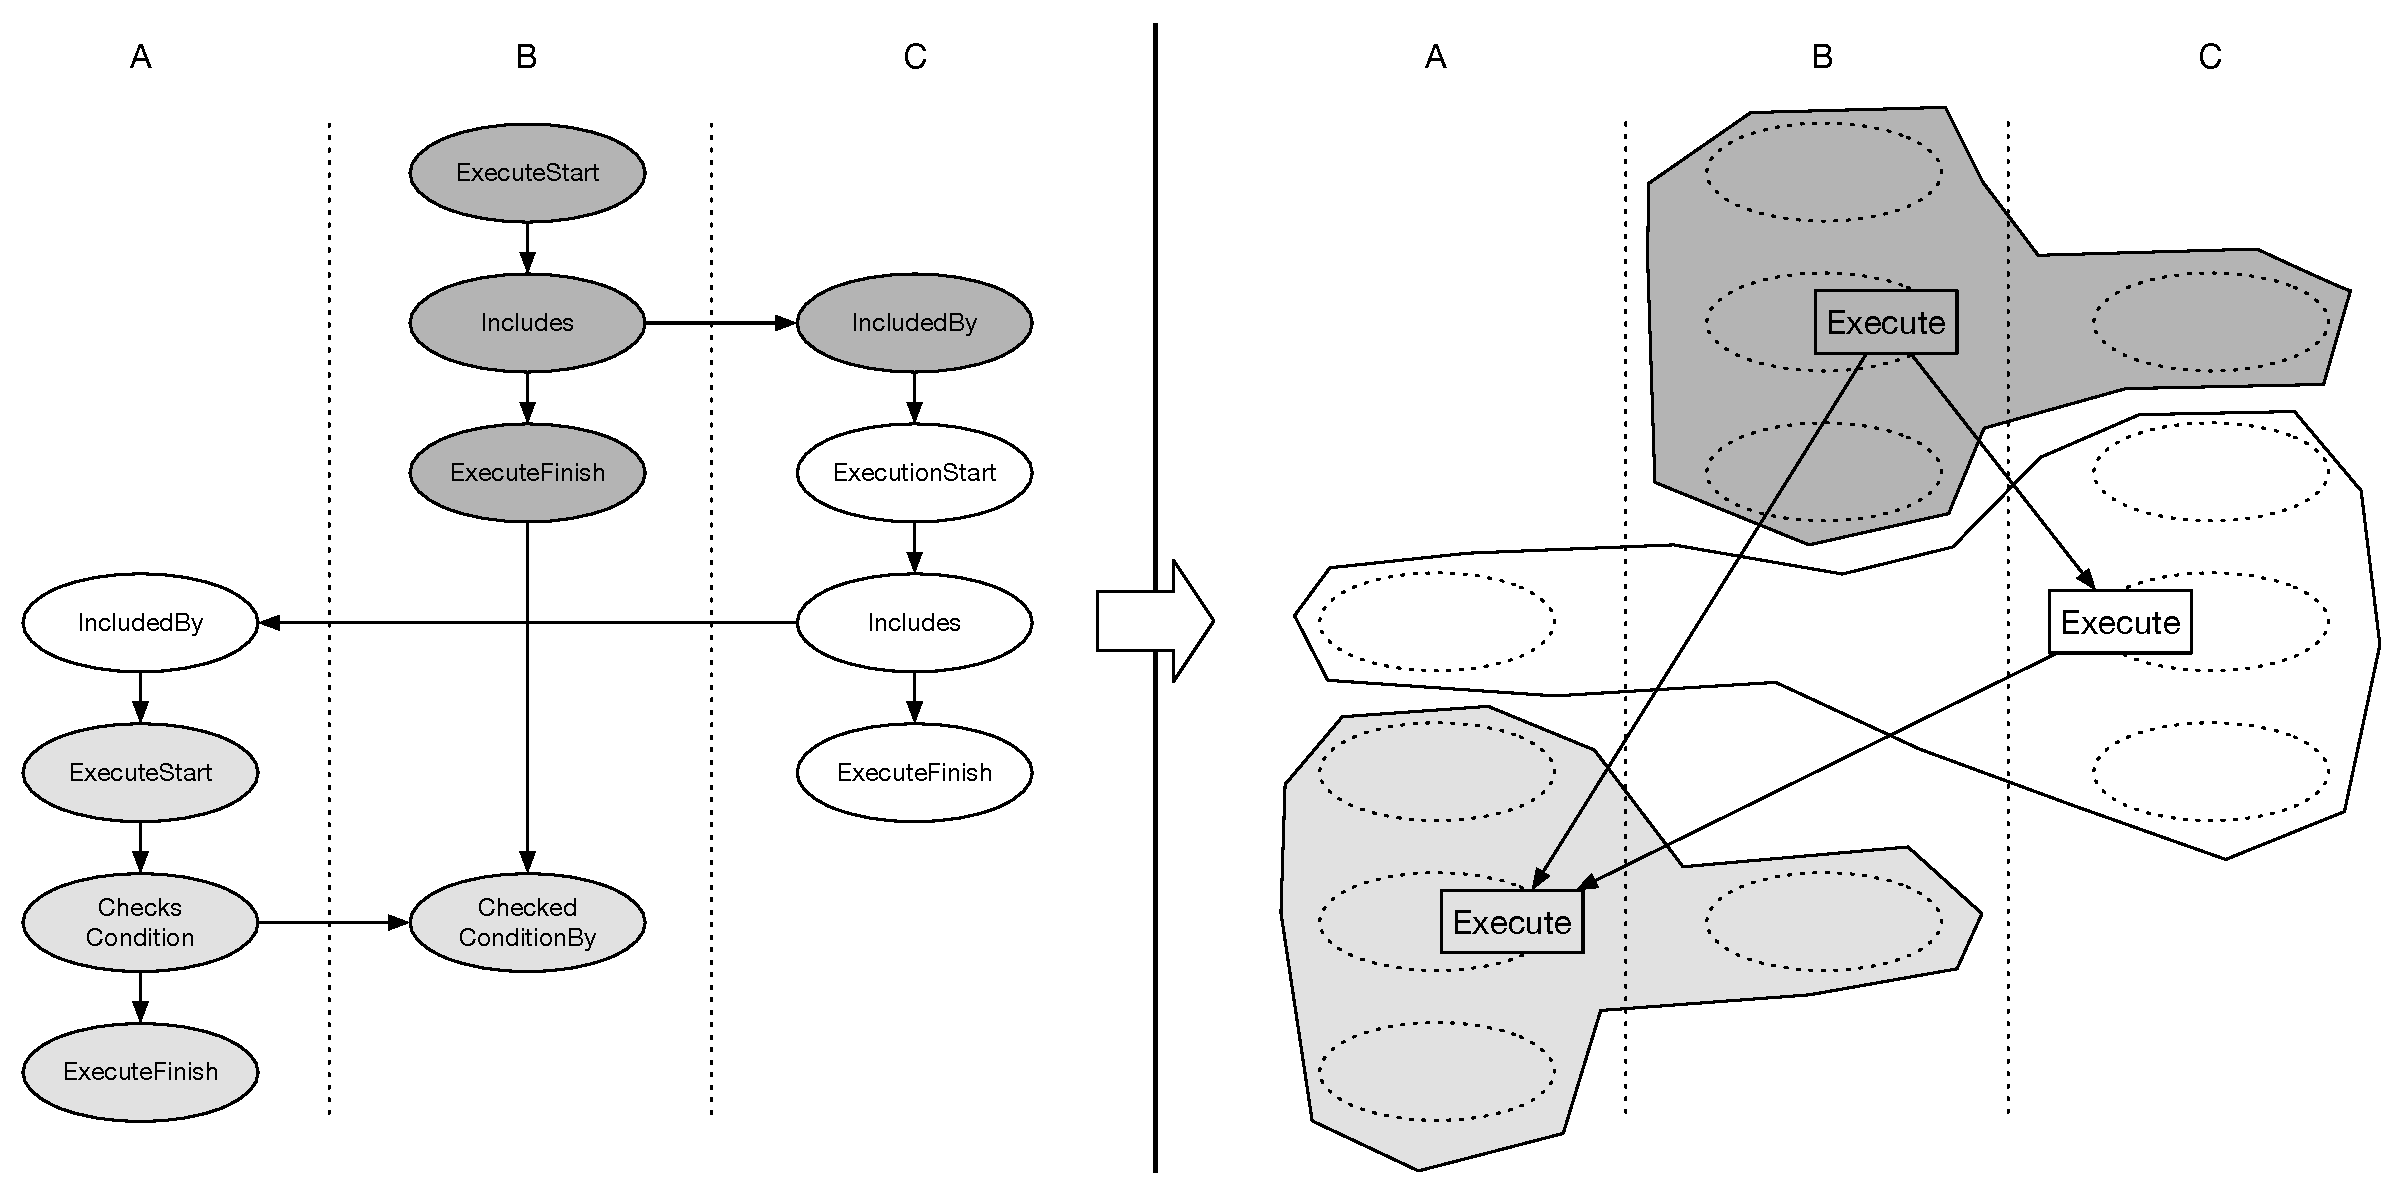
\includegraphics[width=\textwidth]{6orderofexecution/images/transitive-example-collapse.pdf}
		\caption{The result of collapsing actions in the histories of three events.}
		\label{fig:orderofexecution:collapsing}
	\end{figure}
	
	\begin{figure}
		\centering
		\def\svgwidth{0.42\columnwidth}
		\fontsize{6}{8}\selectfont
		\import{4connect/images/}{before_collapsing.pdf_tex}
		\caption{Separation of executions}
		\label{fig:before-collapsing}
	\end{figure}
	\todo{Denne figur skal laves ud fra GasWorkflow.}
	
	\newpar When actions contained in an execution have been found, it is necessary to decide what should happen to the grouping of the actions. It is desired to keep all relations intact, to avoid modifying the history and only simplify it. 
	
	By pointing all ingoing edges to the current event towards a new \textit{collapsed node}, and adding all outgoing edges to the new node, this is accomplished. This new \textit{collapsed node} then represents the entire execution. 
	
	In the implemented solution the the \texttt{ExecuteFinish} type has been chosen to denote a collapsed execution in order to avoid creating a new action type. As it can be seen in \autoref{fig:after-collapsing} the collapsing of executions results in an order of execution.
	\todo{udvid (find bedre eksempel) med at særlige tilfælde kræver transitive reduction efter\-følgende}
	
	\begin{figure}
		\centering
		\def\svgwidth{0.22\columnwidth}
		\fontsize{6}{8}\selectfont
		\import{4connect/images/}{after_collapsing.pdf_tex}
		\caption{Executions after collapsing}
		\label{fig:after-collapsing}
	\end{figure}
	\todo{Denne figur skal laves ud fra GasWorkflow.}
	
	The Collapse algorithm can be seen in \autoref{alg:collapse}.
	
	\begin{algorithm}
		\begin{algorithmic}
			\Function{Collapse}{graph}\State
				locals: CollapseMap: Mapping from old to newaction IDs.
				\State\hspace{28pt} Result: Graph, initially empty
				\State
				\State ExecuteStarts $\leftarrow$ \Call{Filter}{type = ExecuteStart, graph} \State
				Executions $\leftarrow$ \Call{Map.map}{FindSingleExecution, ExecuteStarts}
				\ForAll{executions in Executions}\State
					CollapseMap $\leftarrow$ \Call{CreateExecutionMap}{execution, newExecutionId, CollapseMap}
				\EndFor
				\ForAll{oldActionID, newActionID in CollapseMap}
					\State
					NewAction $\leftarrow$ Action with \State\hspace{28pt}ID = newActionID and \State\hspace{28pt}Edges = edges from oldActionID in graph mapped to new IDs\State
					Result $\leftarrow$ \Call{AddNode}{NewAction, Result} \State\Comment{This requires AddNode to merge edge sets when existing nodes are added}
				\EndFor
				
			\EndFunction
			\State
			\Function{FindSingleExecution}{startAction}
				\State locals: execution
				\While{startAction.Type $\neq$ ExecuteFinish} \State
					execution $\leftarrow$ \Call{AddRange}{startAction.Edges, execution}
				\EndWhile\State
				\Return execution
			\EndFunction
			\State
			\Function{CreateExecutionMap}{ActionSet, newActionId, accumulatorMap}
				\ForAll{actions in ActionSet}\State
					accumulatorMap $\leftarrow$ \Call{Add}{action.Id, newActionId, accumulatorMap}
				\EndFor \State
				\Return accumulatorMap
			\EndFunction
		\end{algorithmic}
		\caption{Collapse algorithm}
		\label{alg:collapse}
	\end{algorithm}
	
%    \subsection{Correctnes}
	The found order of execution still represents the same history and have the same properties as to the order. Given the definition of serially equivalence, which executions complies with, two processes happen after one another. Therefore the set of actions which are after actions in an execution must happen after that execution finishes, just as well as all action which happen before actions in an execution must happen before the execution starts. 

    
	\subsection{Transitive Reduction}
	
	\newpar Redundant edges might still exist in the history after executions of the history have been collapsed. An edge is redundant in cases where there exists a path from an execution to another execution through another execution, but there also exists a direct edge between the two executions. In this case the direct edge is redundant and can be removed, since it does not contribute extra information in regards to the ordering of the executions, and removing it will not affect the ordering or reachability of the order of execution, but rather simplify the order of execution.
	
	\newpar An example of a redundant edge in a collapsed order of execution can be seen in figure \autoref{fig:orderofexecution:collapsing}. The figure illustrates a case where a redundant edge exists between event $A$ and event $B$, since the edge from event $B$ through $C$ provides more information about the order in which the executions occurred.  
	
	\newpar Recall that the order of execution is represented as a directed acyclic graph. For a directed acyclic graph a subgraph of the graph with the same ordering and reachability, but as few edges as possible, can be found, called a \textit{minimum equivalent graph}. 
	
	In directed acyclic graphs the transitive reduction of a given graph is a graph with the fewest possible number of edges, but the same reachability as the given graph. 
	
	That is, if there exists a path from an edge $x$ to an edge $y$ in graph G, there must also be a path from $x$ to $y$ in the transitive reduction of $G$, and vice versa.
	
	Furthermore, the transitive reduction will always be a subgraph of the given graph. For that reason the transitive reduction corresponds to the minimum equivalent graph.  
	
	\todo[inline]{Måske skal disse to paragraffer smeltes sammen? Det er to forskellige concepter, der dog er lig hinanden i DAC's, og de resulterer dermed i det samme..}
	
	\newpar Finding the transitive reduction of the order of execution is desired, since this results in the simplest possible order of execution where reachability is preserved. No information is therefore lost, and redundant edges are simply removed. 
	
	The implementation for finding the transitive reduction on an order of execution is shown in \autoref{alg:orderofexecution:reduction}.
	
	\begin{algorithm}[H]
		\begin{algorithmic}
			\Function{Transitive-Reduction}{$history$}
				\ForAll{$execution1$ \textbf{in} $history$}
					\ForAll{$execution2$ \textbf{in} $history$}
						\If{\Call{pathExists}{$execution1$, $execution2$, $history$}}
							\ForAll{$execution3$ \textbf{in} $history$}
								\If{\Call{edgeExists}{$execution2$, $execution3$, $history$}}
									\If{\Call{edgeExists}{$execution1$, $execution3$, $history$}}
										\State $history$ $\leftarrow$ \Call{removeEdge} {$execution1$, $execution3$, $history$}
									\EndIf
								\EndIf
							\EndFor
						\EndIf
					\EndFor
				\EndFor
			\State
			\Return $history$
			\EndFunction
		\end{algorithmic}
		\caption{Transitive Reduction Algorithm}
		\label{alg:orderofexecution:reduction}
	\end{algorithm}
	
	\newpar The shown algorithm for transitive reduction has $O(n^3)$ complexity where $n$ is the number of executions, since the algorithm has three nested for-loops over all executions in the history. This is based on the requirements that $pathExist$ runs in linear time and $edgeExist$ is a constant lookup. In actual use cases the graph will not be totally connected and therefore the innermost loop will not be executed for most executions.
	
	\newpar These algorithms do not provide a way to ensure that malicious nodes cannot tamper with the history. As in the case where one event represented the workflow, there is no way of making sure that the event creating the history will not tamper with the history. It would be possible to pinpoint which neighbouring events are malicious if enough of the neighbours have relations to each other. 

	\section{Election} 
	As we have now found an order of execution where (potentially) malicious events have been identified, we want to know if the remaining events can agree upon the rest of order of execution.
	
	\newpar As stated in the problem definition, it is desired to reach consensus on the resulting order of execution, but since no process in the system knows the entire state of a workflow, it is not possible for the events to suggest an order of execution without completing steps alike with the ones described in this report.
	
	\newpar Because we have chosen to let the client know all events in order to retrieve their histories, it is also easy for us to send the resulting order of execution back to them, in order to find out whether or not they can agree to this order.
	
	\newpar When any event receives this order of execution, it can look at its own history and at the received order. In a good event the local history can contain executions with outgoing actions between execute start and execute finish actions. Furthermore ingoing relations can be identified as executions of other events from the following rules:
	
	\begin{itemize}
		\item Each counterpart present in actions with ingoing action types must have executed at least once, in order to contact the local event.
		\item If two actions with the same ingoing action type and counterpart are present after each other, this denotes two separate executions of the counterpart event, because each executing event only contacts another event once per relation when executing.
	\end{itemize}
	
	\newpar Furthermore if an event has sent multiple ingoing requests as part of a single execution, then each of the relations that these actions represent must be present every time that execution has happened. Given these rules, the local history can be turned into a "local order of execution".
	
	\newpar In order for the event to agree on the global order of execution, if there exists a path from one execution to another in the local order of execution, there must also exist a path between these executions in the global order of execution.
	
	\newpar \todo[inline]{Hvordan bruger vi det her til at skrive at election i virkeligheden er en bekræftelse af vores algoritme, mere end det er en egentlig afstemning om resultatet?}